\chapter{Esperimenti}\label{ch:experiments}

Per confrontare le varie modalit\`a e avere una misura di quali siano le migliori non possiamo basarci solamente su analisi generali, ma dobbiamo fare degli esperimenti.

Per gli esperimenti verranno usate come confronti le lettere in figura \ref{fig:letters}.

\begin{figure}
    \centering
    \begin{tabular}{c|c|c}
        & \emph{d} & \emph{s} \\ \hline
        dritta 
        & 
        \begin{minipage}{.3\textwidth}
            \centering
            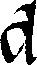
\includegraphics{figures/D_dritta.png}
        \end{minipage}
        & 
        \begin{minipage}{.3\textwidth}
            \centering
            
\includegraphics{figures/S_dritta.png}
        \end{minipage}
        \\ \hline
        tonda 
        & 
        \begin{minipage}{.3\textwidth}
            \centering
            
\includegraphics{figures/D_tonda.png}
        \end{minipage}
        & 
        \begin{minipage}{.3\textwidth}
            \centering
            
\includegraphics{figures/S_tonda.png}
        \end{minipage}
        
    \end{tabular}
    \caption{Le lettere usate come confronto.}
    \label{fig:letters}
\end{figure}

Per valutare le prestazioni di ciascun algoritmo in maniera automatica viene usato un file .json che accompagna la scannerizzazione dell'immagine. In tale file ci sono indicate delle coordinate per ciascuna lettera di interesse. Per avere un unico punto associato a ciascuna lettera, si trova il punto medio fra quelli forniti, in modo da essere sicuri che questo sia in un punto interno alla lettera.

Per trovare le lettere nel testo viene usata una funzione che riceve in ingresso un immagine sezionata secondo le modalit\`a descritte alla sezione \ref{sect:segmentation}, l'immagine della lettera usata come confronto, l'indice di Jaccard da prendere come valore di soglia e un valore per indicare che modalit\`a usare. Questa funzione dovr\`a dunque restituire una lista di rettangoli che sono i rettangoli contenenti le lettere che superano il test e i relativi valori di Jaccard. Ciascun rettangolo sar\`a rappresentato come una coppia di coordinate che si riferiscono a una coppia di vertici opposti.

\section{Grafici precision recall}

Una volta che abbiamo le rappresentazioni di tutti i rettangoli che l'algoritmo ritiene siano la lettera cercata, possiamo usare la lista di coordinate associate alle lettere corrette per quantificare gli errori dell'algoritmo. In particolare dobbiamo contare le volte in cui l'algoritmo ha creduto che una lettera fosse la stessa del riferimento sbagliandosi (falsi positivi) e le volte in cui ha creduto che una lettera non fosse la stessa del riferimento sbagliandosi (falsi negativi).

Idealmente vorremmo che sia i falsi positivi che i falsi negativi fossero 0. Tuttavia ci\`o \`e difficile da ottenere, in quanto alzando il valore di indice di Jaccard di soglia aumentano i falsi negativi, mentre abbassandolo aumentano i falsi positivi.

Nelle figure da \ref{fig:graph_D_dritta} a \ref{fig:graph_S_tonda} si possono visualizzare le affermazioni fatte precedentemente (i grafici relativi alla connettivit\`a a 8 sono stati omessi perch\'e troppo simili ai corrispondenti per la connettivit\`a a 4). Nei grafici sull'asse delle ascisse c'\`e il recall (o sensibilit\`a) e sull'asse delle ordinate la precision (o predittivit\`a). Le definizioni di queste misure sono date in termini dei veri positivi $V_+$, i falsi positivi $F_+$, i veri negativi $V_-$ e i falsi negativi $F_-$.

\begin{equation*}
    \text{recall} = \frac{V_+}{V_+ + F_-}
\end{equation*}

\begin{equation*}
    \text{precision} = \frac{V_+}{V_+ + F_+}
\end{equation*}

Ci\`o che si deduce da queste definizioni \`e che il recall \`e una misura degli errori intesi come falsi negativi, mentre la precision \`e una misura degli errori intesi come falsi positivi. Il caso ideale sarebbe avere precision e recall entrambi pari ad uno. Dai grafici \`e possibile confrontare i vari metodi per cercare di capire quale sia il migliore, ovvero quello che approssima meglio la curva ideale passante da $(1, 1)$.

\begin{figure}
    \centering
    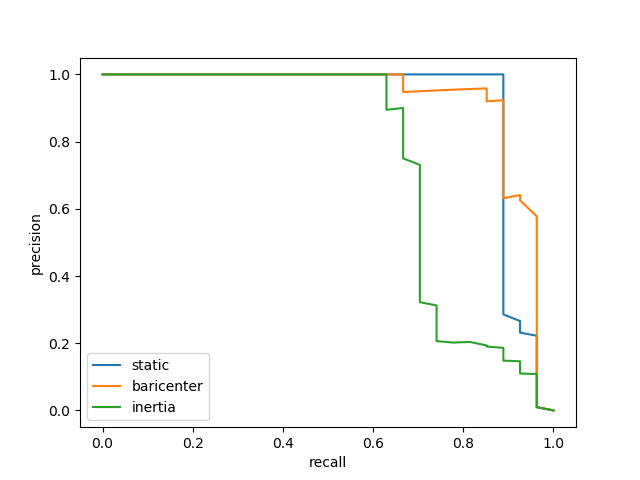
\includegraphics[width=.9\textwidth]{figures/graphs/D_drittaFalse.png}
    \caption{Curve di precision recall per la \emph{d} dritta usando la connettivit\`a a 4.}
    \label{fig:graph_D_dritta}
\end{figure}

\begin{figure}
    \centering
    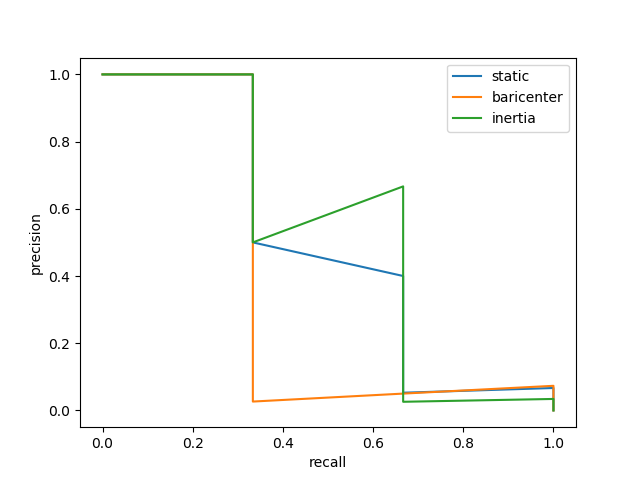
\includegraphics[width=.9\textwidth]{figures/graphs/D_tondaFalse.png}
    \caption{Curve di precision recall per la \emph{d} tonda usando la connettivit\`a a 4.}
    \label{fig:graph_D_tonda}
\end{figure}

\begin{figure}
    \centering
    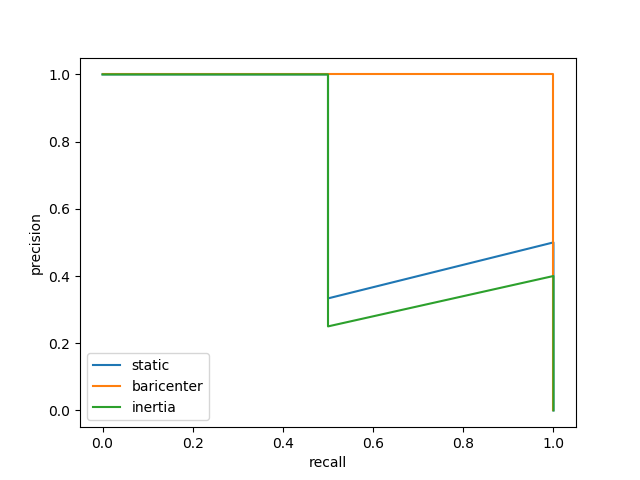
\includegraphics[width=.9\textwidth]{figures/graphs/S_drittaFalse.png}
    \caption{Curve di precision recall per la \emph{s} dritta usando la connettivit\`a a 4.}
    \label{fig:graph_S_dritta}
\end{figure}

\begin{figure}
    \centering
    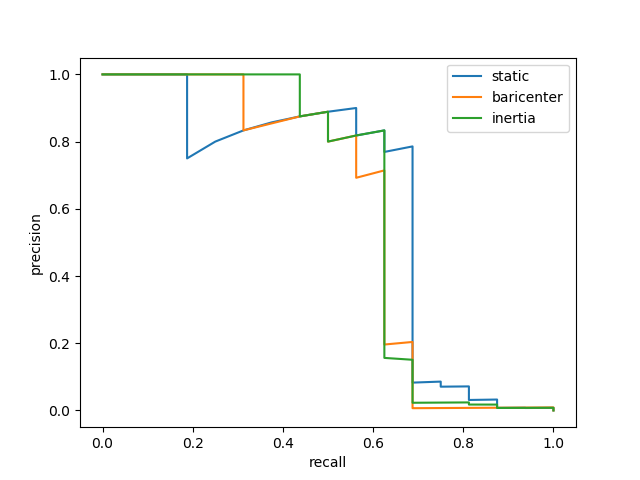
\includegraphics[width=.9\textwidth]{figures/graphs/S_tondaFalse.png}
    \caption{Curve di precision recall per la \emph{s} tonda usando la connettivit\`a a 4.}
    \label{fig:graph_S_tonda}
\end{figure}

\section{Precision interpolata}

I grafici possono essere semplificati facendone quella che viene chiamata interpolazione. In pratica ci si accorge che per alcuni tratti il grafico va ``in salita'', ovvero passa da un punto ad un altro con maggiore recall e precision. Questo significa che il secondo punto \`e migliore al primo secondo ogni misura. Detta in altri termini, usare il valore di soglia per l'indice di Jaccard relativo al secondo punto rispetto a quello del primo punto, comporta l'esclusione di grafemi incorretti, ma non di grafemi corretti e quindi \`e preferibile indiscutibilmente.

Di conseguenza possiamo fare in modo che il primo punto erediti la precision del secondo, in modo da passare dal grafico che indica ``il miglior valore di precision ottenibile per un valore di recall pari a $x$'' a quello che indica ``il miglior valore di precision ottenibile per un valore di recall pari \emph{o maggiore} di $x$''. In questo modo si capisce bene che il grafico interpolato \`e pi\`u interessante.

Formalmente la precision nel grafico interpolato si trova come:
\begin{equation*}
    p_{interp}(r) = \max_{r' \geq r} p(r')
\end{equation*}
Dove $p_{interp}$ \`e la precision interpolata, $p$ la precision, e $r$ un valore di recall.

Nelle figure da \ref{fig:graph_D_dritta_interpolated} a \ref{fig:graph_S_tonda_interpolated} viene raffigurata la versione interpolata dei grafici precision recall.

\begin{figure}
    \centering
    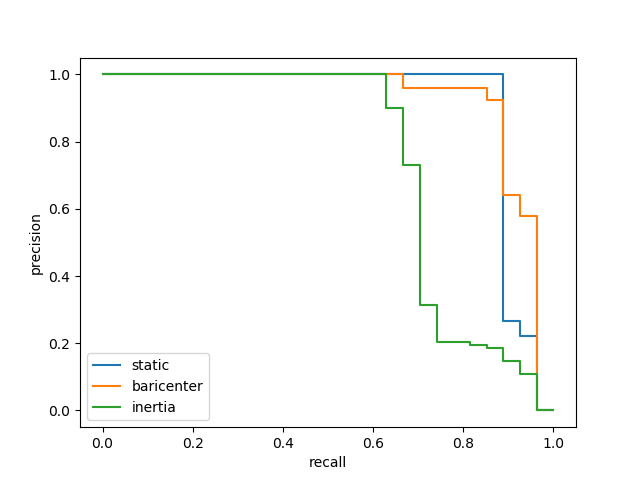
\includegraphics[width=.9\textwidth]{figures/graphs/D_drittaFalseinterpolated.png}
    \caption{Curve di precision recall interpolate per la \emph{d} dritta.}
    \label{fig:graph_D_dritta_interpolated}
\end{figure}

\begin{figure}
    \centering
    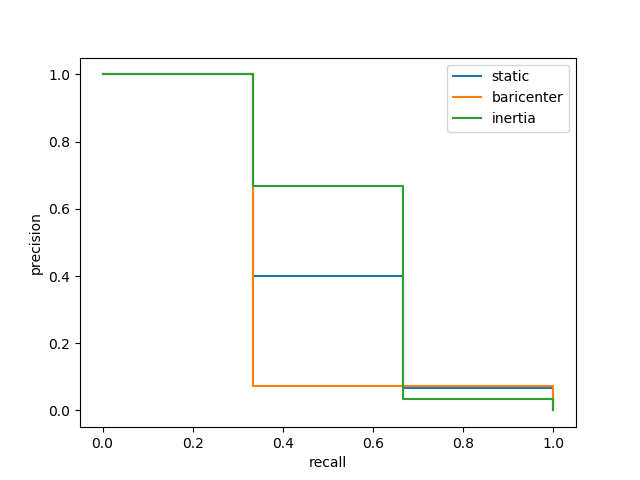
\includegraphics[width=.9\textwidth]{figures/graphs/D_tondaFalseinterpolated.png}
    \caption{Curve di precision recall interpolate per la \emph{d} tonda.}
    \label{fig:graph_D_tonda_interpolated}
\end{figure}

\begin{figure}
    \centering
    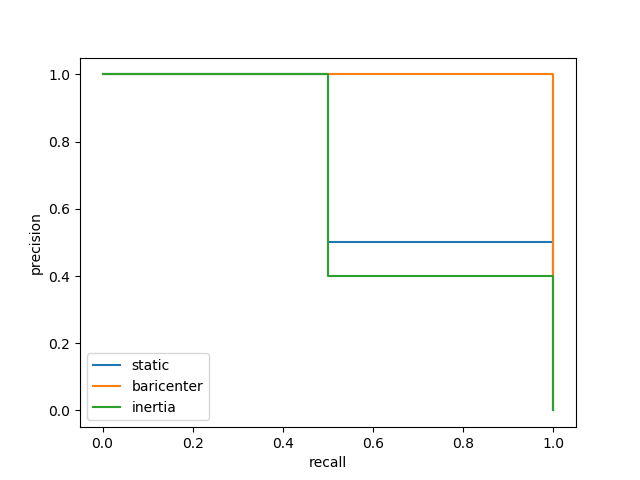
\includegraphics[width=.9\textwidth]{figures/graphs/S_drittaFalseinterpolated.png}
    \caption{Curve di precision recall interpolate per la \emph{s} dritta.}
    \label{fig:graph_S_dritta_interpolated}
\end{figure}

\begin{figure}
    \centering
    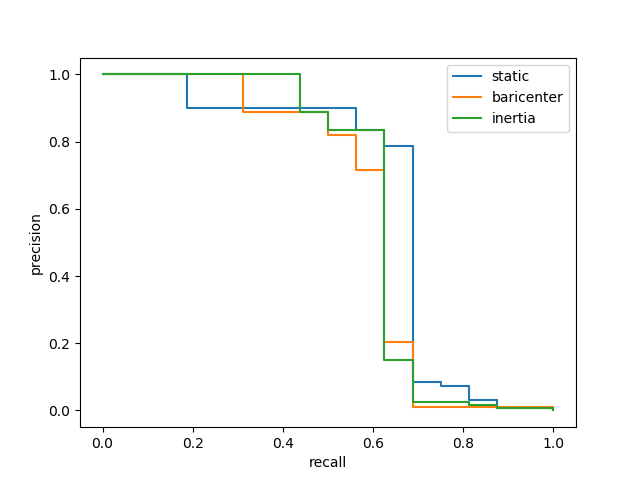
\includegraphics[width=.9\textwidth]{figures/graphs/S_tondaFalseinterpolated.png}
    \caption{Curve di precision recall interpolate per la \emph{s} tonda.}
    \label{fig:graph_S_tonda_interpolated}
\end{figure}

\section{Media fra grafici}

Usare quattro grafici per descrivere un unico metodo \`e eccessivo e dovremmo condensarli in un unico grafico per poter confrontare i metodi pi\`u facilmente. Per fare ci\`o possiamo fare una media fra i grafici delle varie lettere ottenuti con lo stesso metodo per poi confrontare queste medie.

La media non deve essere una media aritmetica standard, poich\'e darebbe eguale peso a tutti i grafemi. Dobbiamo utilizzare una media pesata dove il peso di ciascun grafema \`e dato dalla sua frequenza nel testo. Utilizzando questo approccio, i grafici che otteniamo sono quelli nella figura \ref{fig:graph_all}. Come si evince dalle figure, e come \`e facilmente dimostrabile, la media fra grafici interpolati \`e a sua volta un grafico interpolato e quindi non \`e necessario farne l'interpolazione.

\begin{figure}
    \centering
    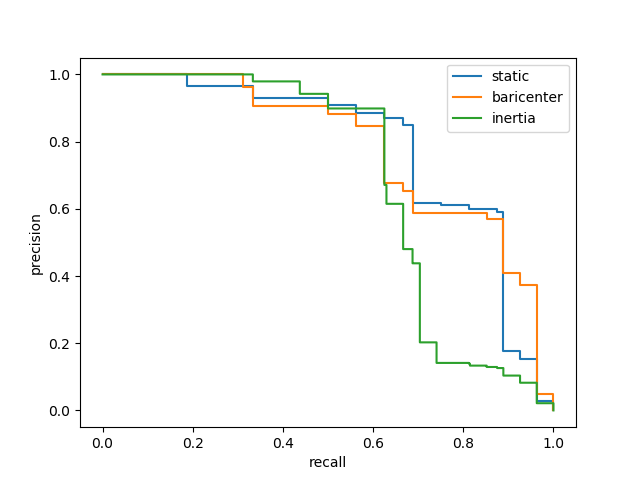
\includegraphics[width=\textwidth]{figures/graphs/False.png}
    \caption{Curve di precision recall medie.}
    \label{fig:graph_all}
\end{figure}

Da questi grafici possiamo notare che il metodo inerziale \`e il migliore per recall bassi, il metodo del baricentro \`e il migliore per recall alti, e il metodo statico \`e il migliore per recall intermedi.

\section{Area}

Dai grafici, anche da quelli complessivi, \`e difficile capire quale metodo sia il migliore in generale. Quello che possiamo fare in questi casi \`e passare da un grafico ad un unico numero. Un modo per fare questo \`e calcolare l'area sottesa dal grafico. Quest'area sar\`a un valore compreso fra 0 e 1 e a metodi migliori corrisponderanno aree maggiori.

Le aree sono facilmente calcolate poich\'e sono semplicemente somme di aree di rettangoli. I loro valori sono riportati in tabella \ref{tab:area}. Come si pu\`o notare i metodi corrispondono a aree simili, tutte vicine a $0.78$, fatta eccezione per il metodo inerziale. Questo \`e probabilmente dovuto al fatto che le lettere sono tutte delle stesse dimensioni, mentre il metodo inerziale \`e efficacie quando le dimensioni sono variabili.

\begin{table}
    \centering
    \begin{tabular}{c|c|c}
        metodo & connettivit\`a 4 & connettivit\`a 8 \\
        \hline
        centrale & \textbf{0.785} & 0.784 \\
        baricentro & 0.782 & 0.781 \\
        inerzia & 0.685 & 0.681 \\
    \end{tabular}
    \caption{Le aree sotto le curve precision recall per tutti i metodi testati. \`E stato evidenziato il valore massimo.}
    \label{tab:area}
\end{table}